\documentclass[pdf]{beamer}

\usepackage[utf8]{inputenc}
\usepackage[brazil]{babel}
\usepackage{graphicx}
\usepackage[normalem]{ulem}
\usepackage{listings}
\usepackage{hyperref}

\hypersetup{colorlinks=true,linkcolor=blue,urlcolor=blue,citecolor=blue,anchorcolor=blue}

\lstset{breakatwhitespace,
  language=C,
  columns=fullflexible,
  keepspaces,
  breaklines,
  tabsize=4,
  showstringspaces=false,
  extendedchars=true,
  keywordstyle=\color{blue}\ttfamily,
  stringstyle=\color{red}\ttfamily,
  commentstyle=\color{green!40!black}\ttfamily,
  morecomment=[l][\color{magenta}]{\#}
}

\lstset{breakatwhitespace,
  language=Python,
  columns=fullflexible,
  keepspaces,
  breaklines,
  tabsize=4,
  showstringspaces=false,
  extendedchars=true,
  keywordstyle=\color{blue}\ttfamily,
  stringstyle=\color{red}\ttfamily,
  commentstyle=\color{green!40!black}\ttfamily,
  morecomment=[l][\color{magenta}]{\#}
}

\usetheme{progressbar}

\title[PyUSB]{Easy USB device access}
\subtitle{with PyUSB}

\author{{\Large Wander Lairson Costa}}
\institute{{\large Mozilla Corporation}}

\date{}

\begin{document}

\begin{frame}
  \titlepage
  \begin{center}
    \begin{tabular}{c}
      \url{https://twitter.com/walac00} \\
      \url{https://github.com/walac} \\
      \url{https://walac.github.io} \\
      \url{https://br.linkedin.com/in/walac} \\
      \href{mailto:wander.lairson@gmail.com}{wander.lairson@gmail.com} \\
    \end{tabular}
  \end{center}
\end{frame}

\begin{frame}{USB Introduction}
  \begin{center}
    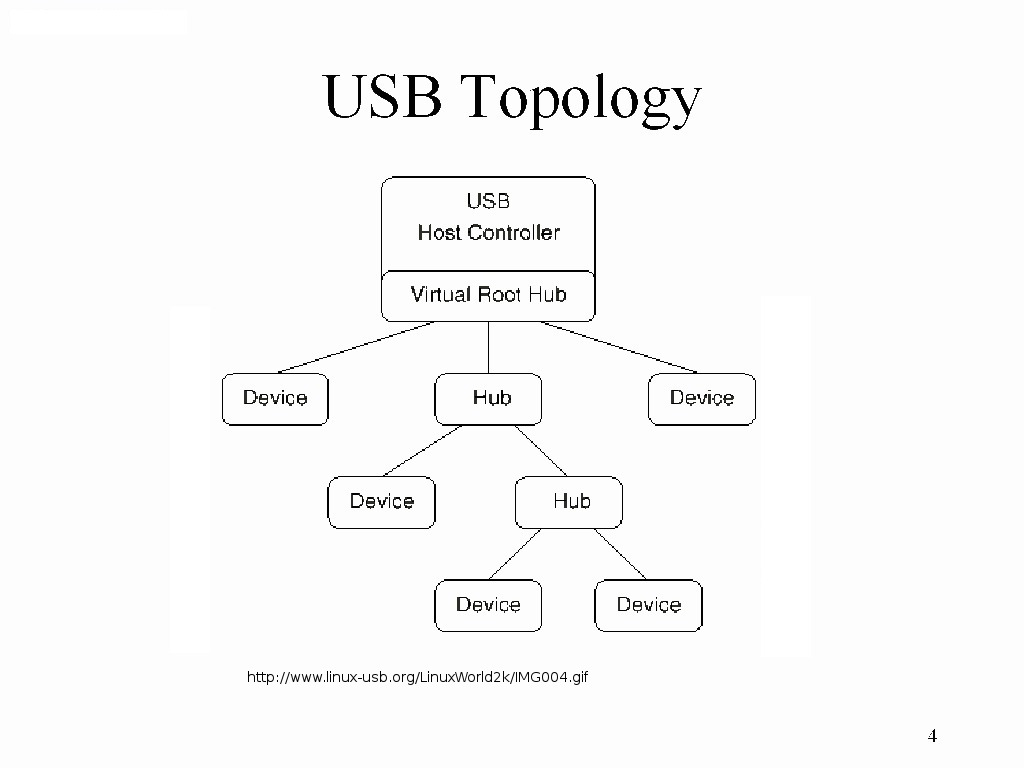
\includegraphics[scale=0.15]{img/topology.jpg}
  \end{center}
  \begin{itemize}
    \tiny
    \item Universial Serial Bus
    \item Created to replace several slow connections (serial, parallel, etc)
    \item It is hot plug and play bus. You don't need to turn off your computer
        connect a new device.
    \item It works as a Master/Slave. All requests are initiated by the Host (polling).
    \item USB 3.1 can reach up to 1GB/s transfer rates
  \end{itemize}
\end{frame}

\begin{frame}{USB Descriptors}
  \begin{center}
    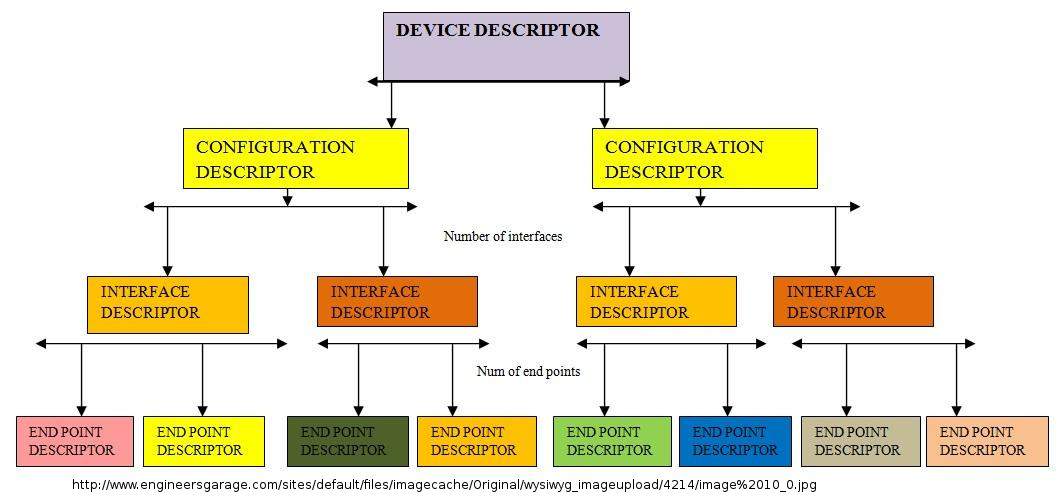
\includegraphics[scale=0.3]{img/descriptors.jpg}
  \end{center}
\end{frame}

\begin{frame}{Device Descriptor}
  Contains basic information about the device.
  \begin{table}
    \tiny
    \begin{tabular}{| c | c | c | l |}
      \hline
      \textbf{Offset} & \textbf{Field} & \textbf{Size} & \textbf{Description} \\ \hline \hline
      0 & \texttt{bLength} & 1 & Descriptor size \\ \hline
      1 & \texttt{bDescriptorType} & 1 & The device constant (0x01) \\ \hline
      2 & \texttt{bcdUSB} & 2 & USB version number (BCD) \\ \hline
      4 & \texttt{bDeviceClass} & 1 & Class code \\ \hline
      5 & \texttt{bDeviceSubClass} & 1 & Subclass code \\ \hline
      6 & \texttt{bDeviceProtocol} & 1 & Protocol code \\ \hline
      7 & \texttt{bMaxPacketSize0} & 1 & Maximum Packet for Endpoint 0 \\ \hline
      8 & \texttt{idVendor} & 2 & Vendor ID \\ \hline
      10 & \texttt{idProduct} & 2 & Product ID \\ \hline
      12 & \texttt{bcdDevice} & 2 & Device version (BCD) \\ \hline
      14 & \texttt{iManufacturer} & 1 & Manufacturer string descriptor index \\ \hline
      15 & \texttt{iProduct} & 1 & Product string descriptor index \\ \hline
      16 & \texttt{iSerialNumber} & 1 & Serial number string descriptor index \\ \hline
      17 & \texttt{bNumConfigurations} & 1 & Number of configuration descriptors \\ \hline
    \end{tabular}
  \end{table}
\end{frame}

\begin{frame}{Configuration Descriptor}
  Dictates how a device will work.
  \begin{table}
    \tiny
    \begin{tabular}{| c | c | c | l |}
      \hline
      \textbf{Offset} & \textbf{Field} & \textbf{Size} & \textbf{Description} \\ \hline \hline
      0 & \texttt{bLength} & 1 & Descriptor size \\ \hline
      1 & \texttt{bDescriptorType} & 1 & The configuration constant (0x02) \\ \hline
      2 & \texttt{wTotalLength} & 2 & The total number of bytes for all descriptors \\ \hline
      4 & \texttt{bNumInterfaces} & 1 & Number of interfaces in the configuration \\ \hline
      5 & \texttt{bConfigurationValue} & 1 & Configuration Identifier \\ \hline
      6 & \texttt{iConfiguration} & 1 & Configuration string descriptor index \\ \hline
      7 & \texttt{bmAttributes} & 1 & Self/bus power and remote wakeup settings \\ \hline
      8 & \texttt{bMaxPower} & 1 & Bus power required, expressed as (maximum miliamperes / 2) \\ \hline
    \end{tabular}
  \end{table}
\end{frame}

\begin{frame}{Interface Descriptor}
  Each interface descriptor represents one logic device.
  An interface can have one or more alternate settings.
  \begin{table}
    \tiny
    \begin{tabular}{| c | c | c | l |}
      \hline
      \textbf{Offset} & \textbf{Field} & \textbf{Size} & \textbf{Description} \\ \hline \hline
      0 & \texttt{bLength} & 1 & Descriptor size \\ \hline
      1 & \texttt{bDescriptorType} & 1 & The interface constant (0x04) \\ \hline
      2 & \texttt{bInterfaceNumber} & 1 & The number identifying this interface \\ \hline
      3 & \texttt{bAlternateSetting} & 1 & Value used to select an alternate setting \\ \hline
      4 & \texttt{bNumEndopoints} & 1 & Number of endpoints, not counting Endpoint 0 \\ \hline
      5 & \texttt{bInterfaceClass} & 1 & Class code \\ \hline
      6 & \texttt{bInterfaceSubClass} & 1 & Subclass code \\ \hline
      7 & \texttt{bInterfaceProtocol} & 1 & Protocol code \\ \hline
      8 & \texttt{iInterface} & 1 & Interface string descriptor index \\ \hline
    \end{tabular}
  \end{table}
\end{frame}

\begin{frame}{Endpoint Descriptor}
  An endpoint represents a pipe on the device side to receive data.
  Endpoints, except by Endpoint 0, are unidirectional, and specify
  the data direction from Host point of view.
  \begin{table}
    \tiny
    \begin{tabular}{| c | c | c | l |}
      \hline
      \textbf{Offset} & \textbf{Field} & \textbf{Size} & \textbf{Description} \\ \hline \hline
      0 & \texttt{bLength} & 1 & Descriptor size \\ \hline
      1 & \texttt{bDescriptorType} & 1 & The endpoint constant (0x05) \\ \hline
      2 & \texttt{bEndpointAddress} & 1 & Endpoint number and direction \\ \hline
      2 & \texttt{bmAttributes} & 1 & Transfer type supported \\ \hline
      4 & \texttt{wMaxPacketSize} & 2 & Max packet size supported \\ \hline
      6 & \texttt{bInterval} & 1 & Maximum latency/polling policy interval/NAK rate \\ \hline
    \end{tabular}
  \end{table}
\end{frame}

\begin{frame}{USB Transfers}
  \begin{minipage}{.45\linewidth}
    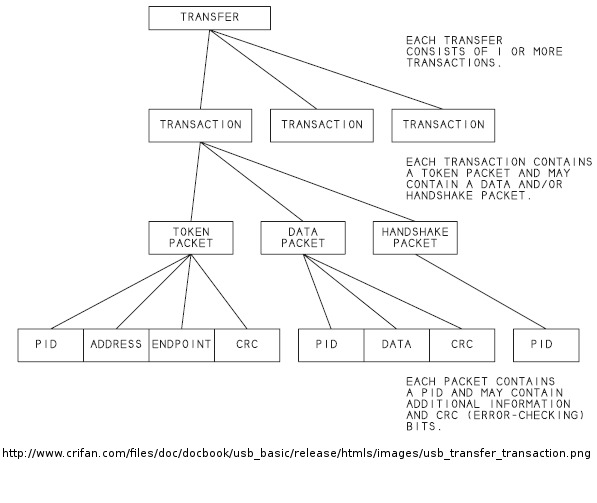
\includegraphics[scale=0.25]{img/usb_transfer.jpg}
  \end{minipage}
  \hspace{.05\linewidth}
  \begin{minipage}{.45\linewidth}
    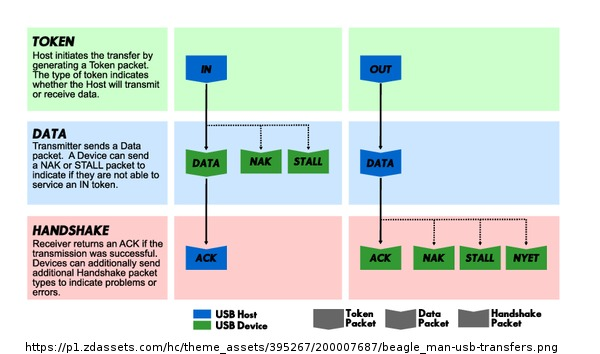
\includegraphics[scale=0.3]{img/usb_transaction.jpg}
  \end{minipage}
\end{frame}

\begin{frame}{Transfer Types}
  \begin{center}
    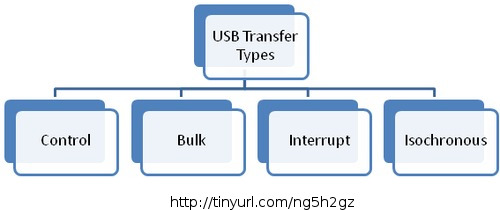
\includegraphics[scale=0.35]{img/transfer_types.jpg}
  \end{center}
  \begin{description}
    \tiny
    \item[Control] used by the Host to configure devices. It is the only transfer
      which supports bidirectional endpoints and which has its format defined by
      the USB spec.
    \item[Bulk] typically used to transfer large amount of data, such as
      printers and disks. The bandwidth allocation can vary, according to the
      bus availability.
    \item[Interrupt] typically used for lower latency, short data transfers. It
      is often used by input devices suchs as mouse and keyboards. Despite its
      name, it works by device polling from the Host.
    \item[Isochronous] used for real time streaming. It prioritizes date rate,
      and it is the only transfer which does not guarantee data delivery, no
      CRC check or retry is performed.
  \end{description}
\end{frame}

\begin{frame}{Accessing USB devices}
  \pause
  Possible solutions:
  \begin{enumerate}
    \pause
    \item Write a kernel device driver.
    \pause
    \item Write a user mode device driver.
    \pause
    \item Use a generic USB library:
      \pause
      \begin{itemize}
          \item libusb 0.1
          \item libusb 1.0
          \item \sout{libusbx}
          \item OpenUSB
          \item libusb-win32
          \item libusbK
      \end{itemize}
      \begin{itemize}
        \pause
        \item Which one to use?
        \pause
        \item PyUSB anwser: anyone!
      \end{itemize}
  \end{enumerate}
\end{frame}

\begin{frame}{PyUSB}
  \begin{itemize}
    \item Up to version 0.4, PyUSB was thin wrapper for libusb 0.1
    \item Starting at version 1.0, PyUSB was redesigned to be a
      platform agnostic, library neutral and easy to use USB access
      package for Python.
    \item PyUSB detaches its API from the backend library used.
    \item You can select the backend you want, but in general PyUSB
      selects the most suitable backend for you.
    \item It works on any Python version $\ge$ 2.4!
    \item 100\% written in Python!
  \end{itemize}
\end{frame}

\begin{frame}[fragile]{Demo:  Listing devices (C Version)}
  \tiny
  \pause
  \begin{lstlisting}[language=C]
    int
    main(void)
    {
      libusb_device **devs;

      libusb_init(NULL);

      const int count = libusb_get_device_list(NULL, &devs);

      for (int i = 0; i < count; ++i)
        dump(devs[i]);

      libusb_free_device_list(devs, 1);
      libusb_exit(NULL);
    }
  \end{lstlisting}
\end{frame}

\begin{frame}[fragile]{Demo:  Listing devices (C Version)}
  \tiny
  \begin{lstlisting}[language=C]
    void
    dump(struct libusb_device *dev)
    {
      struct libusb_device_descriptor desc;
      struct libusb_config_descriptor *cfg;

      libusb_get_device_descriptor(dev, &desc);
      dump_device(&desc);

      for (uint8_t i = 0; i < desc.bNumConfigurations; ++i) {
        libusb_get_config_descriptor(dev, i, &cfg);
        dump_configuration(cfg);
        libusb_free_config_descriptor(cfg);
      }
    }
  \end{lstlisting}
\end{frame}

\begin{frame}[fragile]{Demo:  Listing devices (C Version)}
  \tiny
  \begin{lstlisting}[language=C]
    void
    dump_device(const struct libusb_device_descriptor *dev)
    {
      printf("bcdUSB: %" PRIx16 "\n"
              "bDeviceClass: %" PRIu8 "\n"
              "bDeviceSubClass: %" PRIu8 "\n"
              "bDeviceProtocol: %" PRIu8 "\n"
              "bMaxPacketSize0: %" PRIu8 "\n"
              "idVendor: %" PRIu16 "\n"
              "idProduct: %" PRIu16 "\n"
              "bcdDevice: %" PRIx16 "\n"
              "iManufacturer: %" PRIu8 "\n"
              "iProduct: %" PRIu8 "\n"
              "iSerialNumber: %" PRIu8 "\n",
              dev->bcdUSB,
              dev->bDeviceClass,
              dev->bDeviceSubClass,
              dev->bDeviceProtocol,
              dev->bMaxPacketSize0,
              dev->idVendor,
              dev->idProduct,
              dev->bcdDevice,
              dev->iManufacturer,
              dev->iProduct,
              dev->iSerialNumber);
    }
  \end{lstlisting}
\end{frame}

\begin{frame}[fragile]{Demo:  Listing devices (C Version)}
  \tiny
  \begin{lstlisting}[language=C]
    void
    dump_configuration(struct libusb_config_descriptor *cfg)
    {
      printf("\twTotalLength: %" PRIu16 "\n"
            "\tbNumInterfaces: %" PRIu8 "\n"
            "\tbConfigurationValue: %" PRIu8 "\n"
            "\tiConfiguration: %" PRIu8 "\n"
            "\tbmAttributes: %" PRIx8 "\n"
            "\tMaxPower: %" PRIu8 "\n",
            cfg->wTotalLength,
            cfg->bNumInterfaces,
            cfg->bConfigurationValue,
            cfg->iConfiguration,
            cfg->bmAttributes,
            cfg->MaxPower);

      for (uint8_t i = 0; i < cfg->bNumInterfaces; ++i) {
        const struct libusb_interface *intf = &cfg->interface[i];
        for (int j = 0; j < intf->num_altsetting; ++j)
        dump_interface(&intf->altsetting[j]);
      }
    }
  \end{lstlisting}
\end{frame}


\begin{frame}[fragile]{Demo:  Listing devices (C Version)}
  \tiny
  \begin{lstlisting}[language=C]
    void
    dump_interface(const struct libusb_interface_descriptor *intf)
    {
      printf("\t\tbInterfaceNumber: %" PRIu8 "\n"
              "\t\tbAlternateSetting: %" PRIu8 "\n"
              "\t\tbInterfaceClass: %" PRIu8 "\n"
              "\t\tbInterfaceSubClass: %" PRIu8 "\n"
              "\t\tbInterfaceProtocol: %" PRIu8 "\n"
              "\t\tiInterface: %" PRIu8 "\n",
              intf->bInterfaceNumber,
              intf->bAlternateSetting,
              intf->bInterfaceClass,
              intf->bInterfaceSubClass,
              intf->bInterfaceProtocol,
              intf->iInterface);

      for (uint8_t i = 0; i < intf->bNumEndpoints; ++i)
        dump_endpoint(&intf->endpoint[i]);
    }
  \end{lstlisting}
\end{frame}

\begin{frame}[fragile]{Demo:  Listing devices (C Version)}
  \tiny
  \begin{lstlisting}[language=C]
    void
    dump_endpoint(const struct libusb_endpoint_descriptor *endp)
    {
      printf("\t\t\tbEndpointAdress: %" PRIu8 "\n"
              "\t\t\tbmAttributes: %" PRIx8 "\n"
              "\t\t\twMaxPacketSize: %" PRIu16 "\n"
              "\t\t\tbInterval: %" PRIu8 "\n"
              "\t\t\tbRefresh: %" PRIu8 "\n"
              "\t\t\tbSynchAddress: %" PRIu8 "\n",
              endp->bEndpointAddress,
              endp->bmAttributes,
              endp->wMaxPacketSize,
              endp->bInterval,
              endp->bRefresh,
              endp->bSynchAddress);
    }
  \end{lstlisting}
\end{frame}

\begin{frame}[fragile]{Demo:  Listing devices (Python Version)}
  \tiny
  \pause
  \begin{lstlisting}[language=Python]
    from usb.core import find
    for dev in find(find_all=True):
      print(dev)
  \end{lstlisting}

  \begin{itemize}
    \tiny
    \pause
    \item You can iterate over a descriptor to get inner descritors:
      \begin{lstlisting}[language=Python]
        for cfg in dev:
          print(cfg)

        for intf in cfg:
          print(intf)

        for ep in intf:
          print(ep)
      \end{lstlisting}
    \pause
    \item You can access a inner descriptor by logical index:
      \begin{lstlisting}[language=Python]
        cfg = dev[0]
      \end{lstlisting}
    \pause
    \item You can have more powerful inner descriptors search with
      \texttt{find\_descriptor} function:
      \begin{lstlisting}[language=Python]
        from usb.util import find_descriptor
        cfg = find_descriptor(dev, bConfigurationValue=1)
      \end{lstlisting}
  \end{itemize}
\end{frame}

\begin{frame}[fragile]{Demo: Getting the device serial number (C Version)}
  \tiny
  \pause
  \begin{lstlisting}[language=C]
    #include <libusb.h>
    #include <string.h>

    int main(void)
    {
      libusb_device_handle *handle;
      libusb_device *dev;
      struct libusb_device_descriptor desc;
      int transfered;
      char serial_number[256];

      /* initialized the library */
      libusb_init(NULL);
      atexit(onexit);

      /* open the device */
      handle = libusb_open_device_with_vid_pid(NULL, 0x4d8, 0xfa2e);

      /* get the serial number */
      dev = libusb_get_device(handle);
      libusb_get_device_descriptor(dev, &desc);
      libusb_get_string_descriptor_ascii(handle, desc.iSerialNumber, serial_number, 256);
      printf("Serial number = %s\n", serial_number);

      /* cleanup resources */
      libusb_close(handle);
      libusb_exit(NULL);
    }
  \end{lstlisting}
\end{frame}

\begin{frame}[fragile]{Demo: Getting the device serial number (Python version)}
  \begin{minipage}{.55\linewidth}
    \tiny
    \pause
    \begin{lstlisting}[language=Python]
     from usb.core import find
     dev = find(idVendor=0x4d8, idProduct=0xfa2e)
     print(dev.serial_number)
    \end{lstlisting}
  \end{minipage}
  \hspace{.05\linewidth}
  \begin{minipage}{.35\linewidth}
    \pause
    
\includegraphics[scale=0.15]{img/witchcraft.jpg}
  \end{minipage}

  \begin{itemize}
    \tiny
    \pause
    \item It works with libusb 0.1 and libusb 1.0
    \pause
    \item The \texttt{find} function accepts any device descriptor field
    \pause
    \item \texttt{find} can also return all devices that match the criteria
      (\texttt{find\_all=True} argument).
      \begin{lstlisting}[language=Python]
        devices = find(find_all=True) # all devices
        printers = find(bDeviceClass=7, find_all=True) # all printers
      \end{lstlisting}
    \pause
    \item Use can also specify which backend to use:
      \begin{lstlisting}[language=Python]
        from usb.backend import libusb1
        be = libusb1.get_getbackend()
        dev = find(idVendor=0x4d8, idProduct=0xfa2e, backend=be)
      \end{lstlisting}
  \end{itemize}
\end{frame}

\begin{frame}[fragile]{Demo: Writing data to an endpoint (C version)}
  \tiny
  \pause
  \begin{lstlisting}[language=C]
    #include <libusb.h>
    #include <string.h>

    int main(void)
    {
      libusb_device_handle *handle;
      const char data[] = "test";
      int transfered;

      /* initialized the library */
      libusb_init(NULL);

      /* open the device */
      handle = libusb_open_device_with_vid_pid(NULL, 0x4d8, 0xfa2e);

      /* setup device */
      libusb_set_configuration(handle, 1);
      libusb_claim_interface(handle, 0);

      /* transfer the data */
      libusb_bulk_transfer(handle, 1, data, strlen(data), &transfered, 1000);

      /* cleanup resources */
      libusb_release_interface(handle, 0);
      libusb_close(handle);
      libusb_exit(NULL);
    }
  \end{lstlisting}
\end{frame}

\begin{frame}[fragile]{Demo: Writing data to an endpoint (Python version)}
  \tiny
  \pause
  \begin{lstlisting}[language=Python]
     from usb.core import find
     dev = find(idVendor=0x4d8, idProduct=0xfa2e)
     dev.set_configuration()
     dev.write(1, "test")
  \end{lstlisting}

  \begin{itemize}
    \tiny
    \pause
    \item You don't need to know the endpoint type, PyUSB takes care of it!
    \pause
    \item Reading is as easy as writing:
    \begin{lstlisting}[language=Python]
      data = dev.read(0x81, 4) # return an array.array object
    \end{lstlisting}
    \pause
  \item You can optimize writes and reads using the \texttt{array.array} object directly:
      \begin{lstlisting}[language=Python]
        from array import array
        data = array('B', 'test')
        dev.write(1, data)
        recv = array('B', '\x00'*64)
        bytes_read = dev.read(0x81, recv)
      \end{lstlisting}
  \end{itemize}
\end{frame}

\begin{frame}{More info}
  Future implementations:
  \begin{itemize}
    \item More backends (\texttt{libusbK})
    \item Asynchronous I/O
    \item Hotplug events
  \end{itemize}

  Additional resources:
  \begin{description}
    \item[Project page] \url{https://walac.github.io/pyusb}
    \item[Source code] \url{https://github.com/walac/pyusb}
    \item[Tutorial] \url{https://github.com/walac/pyusb/blob/master/docs/tutorial.rst}
  \end{description}
\end{frame}

\begin{frame}{Thank you!}
  \begin{center}
    
\includegraphics[scale=0.2]{img/questions.jpg}
  \end{center}

  \begin{center}
    \begin{tabular}{c l}
      \textbf{Twitter} & \href{https://twitter.com/walac00}{walac00} \\
      \textbf{Github} & \url{https://github.com/walac} \\
      \textbf{Blog} & \url{https://walac.github.io} \\
      \textbf{Linkedin} & \url{https://br.linkedin.com/in/walac} \\
      \textbf{Email} & \href{mailto:wander.lairson@gmail.com}{wander.lairson@gmail.com} \\
    \end{tabular}
  \end{center}

\end{frame}

\end{document}

